% 1 

\chapter{Wprowadzenie}

\section{Historia systemu operacyjnego Windows}

Na początku lat 80-tych pierwsze komputery osobiste pracowały pod kontrolą systemu operacyjnego
MS-DOS. Swoim użytkownikom DOS oferował prosty interfejs, w którym polecenia systemowe i programy
przywoływało się z {\em linii poleceń}. Programiści mieli do dyspozycji zbiór tzw.{\em przerwań}
za pomocą których mogli sięgać do urządzeń wejścia/wyjścia. DOS był systemem jednozadaniowym,
to znaczy, że w każdej chwili w systemie aktywny był tylko jeden proces\footnote{Pewnym
sposobem na pokonywanie tego ograniczenia było wykorzystanie przerwania zegara, dzięki czemu
było możliwe wykonanie jakiegoś małego fragmentu kodu w regularnych odstępach czasu. Nie zmienia
to jednak faktu, że DOS nie wspierał wielozadaniowości}. 

Pierwsza wersja interfejsu graficznego została zapowiedziana w roku 1983, zaś na rynek trafiła
w listopadzie 1985. Windows 1.0 był odpowiedzią Microsoftu na graficzny interfejs jaki zaprojektowano
w firmie Apple\footnote{Między Microsoftem a Apple regularnie toczyły się spory dotyczące praw
do korzystania z różnych elementów interfejsu graficznego}. W 1987 roku pojawił się Windows 2.0, którego
główną innowacją była możliwość nakładania się okien na siebie (w przeciwieństwie do okien ułożonych obok siebie
w Windows 1.0). Oba systemy pracowały w trybie rzeczywistym procesorów 8086 mając dostęp do 1 MB pamięci.
22 maja 1990 roku pojawił się Windows 3.0, który potrafił już korzystać z trybu chronionego procesora
80386, mając dzięki temu dostęp aż do 16MB pamięci operacyjnej. Dwa lata później, w 1992, pojawił się
Windows 3.1, który wprowadził nowe technologie: czcionki TrueType, OLE oraz obsługę multimediów.
W czerwcu 1993 pojawiła się pierwsza wersja systemu Windows NT, którego jądro pracowało w trybie chronionym
procesorów 80386, liniowym trybie adresowania i 32-bitowym trybie adresowania. Windows NT napisano niemal 
całkowicie od początku w C, dzięki czemu system ten był przenośny i pracował m.in. na platformach RISC-owych.

Wprowadzony na rynek w roku 1995 Windows 95, choć nieprzenośny i uboższy od NT o mechanizmy zabezpieczeń,
zdobył dużą popularność jako system do użytku domowego. Pojawienie się tych dwóch systemów oznacza do dziś
zasadniczą linię podziału Windows na dwie rodziny: rodzinę systemów opartych na jądrze NT (Windows NT, 
Windows 2000, Windows XP) oraz rodzinę opartą na uproszczonym jądrze, rozwijanym od czasów Windows 95
(Windows 95, Windows 98, Windows ME). Zapowiadana kolejna wersja systemu ma ostatecznie połączyć
obie linie.

\section{Windows z punktu widzenia programisty}

System operacyjny Windows zbudowany jest ze współpracujących ze sobą części zarządzających m.in. 
pamięcią, interakcją z użytkownikiem, urządzeniami wejścia-wyjścia. Z punktu widzenia programisty
istotne jest w jaki sposób aplikacja może funkcjonować w systemie 
wchodząc w interakcje z różnymi jego składnikami. To czego potrzebuje programista, to informacje
o tym w jaki sposób aplikacja ma komunikować się z systemem plików, jak obchodzić się z pamięcią, 
jak komunikować się z siecią itd.

Windows jest systemem operacyjnym zbudowanym warstwowo. Tylko najniższe warstwy systemu mogą operować
na poziomie sprzętu - programista takiej możliwości nie ma (poza wczesnymi implementacjami Windows, 
w których taki dostęp jest możliwy). 
Oznacza to, że nie ma możliwości bezpośredniego odwołania się do pamięci ekranu, czy odczytania wartości
z dowolnie wybranej komórki pamięci. Nie można bezpośrednio operować na strukturze dysku twardego, ani
sterować głowicą drukarki. Zamiast tego programista ma do dyspozycji pewien ściśle określony zbiór
{\em funkcji} i {\em typów danych}, za pomocą których program może komunikować się z systemem. 
O takim zbiorze funkcji i typów mówimy, że jest to {\bf interfejs programowania} 
({\em ang. Application Programming Interface, API}) 
jaki dany system udostępnia\footnote{Taka konstrukcja oprogramowania, 
w której wewnętrzne mechanizmy funkcjonowania jakiegoś fragmentu
oprogramowania są ukryte, zaś dostęp do jego funkcji jest możliwy za pomocą jakiegoś interfejsu, 
jest powszechnie stosowany w nowoczesnym oprogramowaniu. Istnieją setki specjalizowanych interfejsów 
programowania przeróżnych bibliotek (DirectX, OpenGL), protokołów (sieć, ODBC, OLEDB), czy programów (MySQL).}.

Dzięki takiej konstrukcji systemu operacyjnego programista nie musi martwić się na przykład o 
model karty graficznej jaki posiada użytkownik, bowiem z jego punktu widzenia oprogramowanie każdego możliwego
typu karty graficznej wygląda dokładnie tak samo. To system operacyjny zajmuje się (tu: za pomocą sterownika)
komunikacją z odpowiednimi częściami komputera i z punktu widzenia programisty robi to w sposób
jednorodny. Co więcej, z punktu widzenia programisty wszelkie możliwe
odmiany systemu operacyjnego Windows, choć bardzo różne "w środku", za zewnątrz wyglądają tak samo. Jeśli
jakaś funkcja występuje we wszystkich odmianach systemu, to jej działanie jest identyczne, choć mechanizmy
jakie pociąga za sobą wywołanie takiej funkcji w systemie operacyjnym mogą być 
zupełnie różne\footnote{Na przykład funkcje do operacji na systemie plików 
czy rejestrze systemu w systemach opartych
na jądrze NT muszą dodatkowo wykonać pracę związaną ze sprawdzaniem przywilejów użytkownika.}.

Od pierwszej wersji systemu Windows, jego interfejs pozostaje w miarę jednolity, mimo że w międzyczasie
przeszedł ewolucję i z systemu 16-bitowego stał się systemem 32-bitowym. Zasadniczo zmienił się
sposób adresowania pamięci (w modelu 16-bitowym odwołania do pamięci miały postać
{\em segment:offset} i były następnie tłumaczone na adersy fizyczne, model 32-bitowy zakłada
32-bitowe liniowe adresowanie pamięci, wykorzystujące odpowiednie możliwości procesorów 80386 i wyższych).
Mimo tej zmiany interfejs programowania pozostał w dużej części nienaruszony. Wszystkie, nawet
najnowsze, wersje systemu, pozwalają na korzystanie zarówno z nowego ({\bf Win32})
jak i starego ({\bf Win16}) interfejsu. Warto wiedzieć, że w systemach opartych na jądrze NT wywołania
funkcji z Win16API przechodzą przez pośrednią warstwę tłumaczącą je na funkcje Win32API obsługiwane
następnie przez system, zaś w systemach opartych na jądrze 16-bitowym 
(Windows 95, Windows 98) jest dokładnie odwrotnie - to funkcje z Win32API przechodzą przez 
warstwę tłumaczącą je na Win16API, które to z kolei funkcje są obsługiwane przez system operacyjny. 
Przyjmuje się że obie linie systemów wspierają Win32API, jednak sytuacja nie jest aż tak różowa -
każdy z systemów obsługuje swój własny podzbiór Win32API. Część wspólna jest jednak na tyle pojemna, że
jak już wcześniej wspomniano, możliwe jest pisanie programów, które działają na każdej odmianie systemu
Windows. 

W pierwszej wersji systemu do dyspozycji programistów oddano około 450 funkcji. W ostatnich wersjach
ich liczba znacząco wzrosła (mówi się o tysiącach funkcji), głównie dlatego, że znacząco wzrosła liczba
możliwości jakimi nowe odmiany systemu dysponują. Każda kolejna warstwa, 
zbudowana nad Win32API, musi z konieczności
być w jakiś sposób ograniczona. MFC, VCL, QT, GTK czy środowisko uruchomieniowe \NETFramework{} 
nie są tu wyjątkami: zdarzają się sytuacje, kiedy zachodzi konieczność sięgnięcia "głębiej" niż pozwalają na to 
wymienione interfejsy, aż do poziomu Win32API. Zrozumienie zasad Win32API pozwala więc przezwyciężać
ograniczenia interfejsów wyższego poziomu\footnote{Tak będziemy mówić o interfejsach zbudowanych na Win32API}.
Pełna dokumentacja wszystkich funkcji systemowych dostępnych we wszystkich interfejsach zaprojektowanych
przez Microsoft oraz mnóstwo artykułów z poradami na temat programowania pod Windows dostępna
jest on-line pod adresem {\em http://msdn.microsoft.com}.

\section{Narzędzia programistyczne} 

Repertuar języków programowania, które pozwalają na pisanie programów pod Windows jest bogaty i każdy
znajdzie tu coś dla siebie. Win32API przygotowano jednak z myślą o języku C i to właśnie pisząc programy 
w języku C można od systemu Windows otrzymać najwięcej. Programiści mają do wyboru nie tylko 
{\em Microsoft Visual C++}, który jest częścią {\em Visual Studio}, ale także kilka niezłych darmowych
kompilatorów rozpowszechnianych na licencji GNU (wśród nich wyróżnia się DevC++, do pobrania ze strony
{\em http://www.bloodshed.net}).

\begin{figure}
\begin{center}
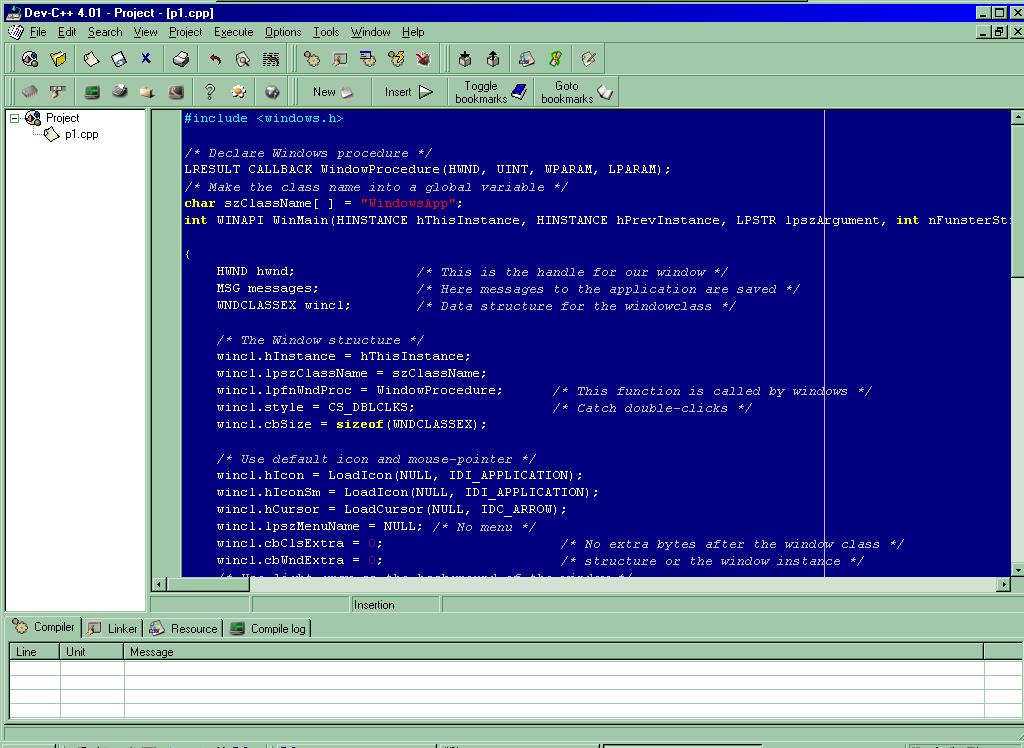
\includegraphics[width=0.75\textwidth]{./pic/w01}
\caption{DevC++ pozwala pisać programy w C i wspiera Win32API.}
\end{center}
\end{figure}

Dużą popularność zdobył sobie język {\em Delphi} zaprojektowany przez firmę {\em Borland} 
jako rozszerzenie {\em Pascala}. Wydaje się jednak, że znaczenie tego języka będzie coraz mniejsze.
Marginalizuje się również znaczenie wielu innych interfejsów takich jak MFC czy VCL.

Pojawienie się języka Java, zaprojektowanego przez firmę Sun, oznaczało dla społeczności programistów
nową epokę. Projektantom Javy przyświecała idea {\em Jeden język - wiele platform}, zgodnie z którą
programy napisane w Javie miały być przenośne między różnymi systemami operacyjnymi. 
W praktyce okazało się, że Java nie nadaje się do pisania dużych aplikacji, osadzonych w konkretnych
systemach operacyjnych. Na przykład oprogramowanie interfejsu użytkownika w Javie polega na skorzystaniu
z komponentów specyficznych dla Javy, nie zaś dla konkretnego systemu operacyjnego. 
Odpowiadając na zarzuty programistów o 
ignorowanie istnienia w systemach operacyjnych specjalizowanych komponentów, Microsoft
przygotował swoją wersję Javy, którą wyposażył w bibliotekę WFC ({\em Windows Foundation Classes}), związującą
{\em Visual J++} z platformą Windows. W 1997 Sun wytoczył Microsoftowi proces, który ostatecznie doprowadził
do zaniechania przez Microsoft rozwijania {\em J++} i podjęcia pracy nad nowym językiem, pozbawionym wad Javy,
który osadzony byłby na nowej platformie, pozbawionej wad środowiska uruchomieniowego Javy. Prace te
zaowocowały pojawieniem się w okoliach roku 2000 pierwszych testowych wersji środowiska uruchomieniowego, 
nazwanego \NETFramework{}, dla którego zaprojektowano nowy język nazwany C\#. Dla wielu programistów 
używających Javy jedną z kropel w kielichu goryczy jest niezgodność semantyczna zachowania się 
maszyn wirtualnych pochodzących z różnych źródeł\footnote{Zdarza się również, że maszyny wirtualne
tego samego producenta zachowują się inaczej na różnych systemach operacyjnych}.

\NETFramework{} opiera się na idei odwrotnej niż Java. Ta idea to {\em Jedna platforma - wiele języków}.
Specyfikacja języka pośredniego, nazwanego {\em IL} ({\em Intermediate Language}) 
jest otwarta dla wszystkich twórców kompilatorów. Co otrzymują w zamian? Wspólny system typów, pozwalający
na komunikację programów pochodzących z różnych języków, rozbudowaną bibliotekę funkcji, wspólny mechanizm
obsługi wyjątków oraz odśmiecacz. Ze swojej strony Microsoft przygotował 5 języków programowania platformy \NET.
Są to:
\begin{itemize}
	\item C\#, w pełni obiektowy język programowania o składni C-podobnej
	\item J++, Java dla platformy \NET
	\item C++, który w nowej wersji potrafi korzystać z dobrodziejstw platformy \NET
	\item VB.NET, nowa wersja Visual Basica o znacznie większych możliwościach niż poprzednia wersja
	\item IL Assembler, niskopoziomowy język programowania w kodzie pośrednim platformy \NET
\end{itemize}

Poza Microsoftem pojawiają się kompilatory innych języków dla platformy \NET. W tej chwili dostępne są
m.in.:
\begin{itemize}
	\item Ada
	\item COBOL
	\item Perl
	\item Python
	\item SmallTalk
	\item SML.NET
\end{itemize}

Trwają prace nad \NET ową wersją Prologa, Delphi oraz wielu innych języków. 

Kompilatory dla trzech języków (C\#, VB.NET, IL Assembler) wchodzą w skład środowiska 
uruchomieniowego \NETFramework, czyli są {\bf darmowe}. Również bez wnoszenia opłat można pobrać ze stron 
Microsoftu pakiet dla J++. 
Sam \NETFramework{} można pobrać również bezpłatnie ze strony
{\em http://msdn.microsoft.com/netframework/downloads/howtoget.asp}. Pakiet instalacyjny zajmuje około
20MB. Programiści mogą pobrać {\em .NET Framework SDK}, który oprócz środowiska uruchomieniowego
zawiera setki przykładów i tysiące stron dokumentacji technicznej. {\em .NET Framework SDK} to około 120MB.
Samo środowisko uruchomieniowe można zainstalować na systemach Windows począwszy od Windows 98. \NETFramework{}
SDK, podobnie jak Visual Studio .NET wymagają już co najmniej Windows 2000, jednak rozwijane 
w Windows 2000 programy dadzą się oczywiście uruchomić w Windows 98 z zainstalowanym 
środowiskiem uruchomieniowym \NET{} (pod warunkiem
nie wykorzystywania klas specyficznych dla Windows 2000, np. {\em FileSystemWatcher}).

Do dyspozycji programistów oddano oczywiście nową wersję środowiska developerskiego {\em Visual Studio .NET}
(oczywiście ono nie jest już darmowe). Dostępne są za to środowiska darmowe, 
rozwijane poza Microsoftem. Najlepiej zapowiada się
{\em SharpDevelop} (do pobrania ze strony {\em http://www.icsharpcode.net}).

\begin{figure}
\begin{center}
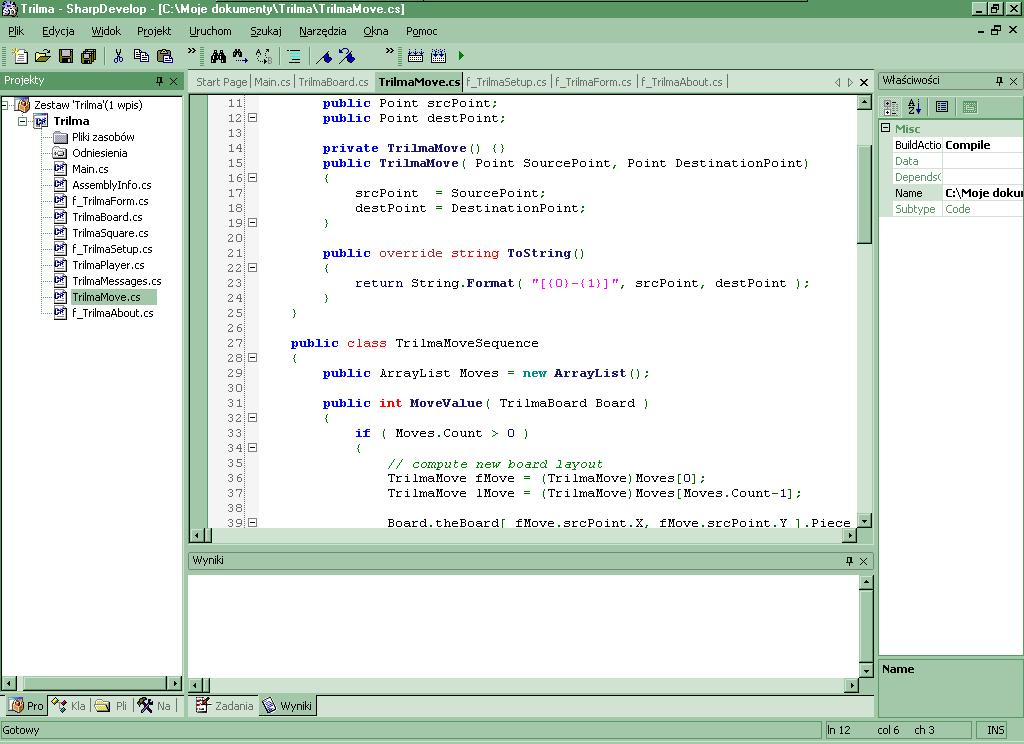
\includegraphics[width=0.75\textwidth]{./pic/w00}
\caption{SharpDevelop oferuje m.in. autouzupełnianie kodu i wizualny edytor form.}
\end{center}
\end{figure}

Specyfikacja platformy \NET{} jest publiczna, ogłoszona poprzez ECMA-International ({\em European Computer
Manufacturer Association International, http://www.ecma-international.org}), nic więc dziwnego, że 
powstają wersje pod inne niż Windows systemy operacyjne. Najbardziej zaawansowany jest w tej chwili
projekt Mono ({\em http://www.go-mono.com}), dostępny na kilka systemów operacyjnych (w tym Linux i Windows).

Platforma \NET{} jest dobrze udokumentowana, powstają coraz to nowe strony, gdzie developerzy
dzielą się przykładowymi kodami i wskazówkami. Warto zaglądać na {\em http://msdn.microsoft.com},
{\em http://www.c-sharpcorner.com}, {\em http://www.gotdotnet.com} czy {\em http://www.codeproject.com}.